\documentclass[Afour,sageh,times,doublespace]{sagej}

\usepackage{amsmath,amssymb}
\usepackage{url}

\def\volumeyear{2026}

\begin{document}

\runninghead{Two Paths Out of Imbalance}

\title{Two Paths Out of Imbalance: How Competing Exits Produce Persistence in Interstate Relations, 1816--2012}

\author{[Author information removed for peer review]}

\begin{abstract}
Why do some inconsistent configurations of interstate alliances and hostilities persist while others rapidly dissolve or realign? Structural balance theory predicts pressure toward consistency but does not specify which of two routes out of imbalance, dissolving or realigning into balance, a given episode takes, or how long that takes. Using signed interstate networks built from Correlates of War alliance and militarized-dispute data, 1816--2012, I identify 6,277 spells of triadic imbalance and model which route each takes with competing-risks hazard models. Greater triadic embeddedness reduces the hazard of dissolution while increasing the hazard of realignment, so persistence concentrates at intermediate embeddedness. Within realigning triads, the tie with the greatest unbalanced load is disproportionately the one that changes, beyond sign and embeddedness alone. Persistence is an emergent consequence of competing resolution routes, not an absence of balance-restoring pressure. Interstate relations are shaped by the triadic structures they are embedded in.
\end{abstract}

\keywords{structural balance, signed networks, militarized disputes, alliance networks, competing risks}

\maketitle

\section*{1. Introduction}

International alliances and militarized disputes do not arrange themselves randomly. A state's formal defense commitments and its militarized disputes are relationally structured, rarely independent of one another, and when a state is simultaneously allied with two states that are themselves rivals, international relations scholars have long treated the resulting configuration as structurally unstable, a source of relational pressure that should, sooner or later, resolve (Maoz et al.~2007). Structural balance theory supplies a formal foundation for that intuition: inconsistent configurations generate pressures that should alter the relationships composing them and move social structure towards greater balance (Heider 1946; Cartwright and Harary 1956). Yet the empirical evidence commonly offered for balance in interstate networks, as elsewhere, is much less dynamic than the theory it supports. Studies frequently establish that balanced configurations are more prevalent than unbalanced ones, or that observed networks contain more balance than appropriate null models would predict (Davis 1967; Maoz et al.~2007). Even this narrower, inferential question has grown more demanding on its own terms, since whether a signed network appears consistent with balance theory at all can depend on which null model is used (Gallo et al.~2024). But however that question is resolved, prevalence evidence of this kind does not show what happens to a particular configuration once it becomes unbalanced, and longitudinal evidence tracing these transitions is scarcer and more mixed. Where it exists, it generally finds unbalanced configurations do not move smoothly toward balance; they can persist, oscillate, or resolve through mechanisms the classical model does not specify (Doreian and Krackhardt 2001). A basic dynamic question at the heart of balance theory therefore remains surprisingly open: what path does imbalance take once it emerges?

Not every unbalanced configuration immediately becomes balanced. Some disappear quickly, others remain inconsistent for years, and still others undergo substantial relational realignment. The persistence of imbalance is particularly important. If inconsistency generates pressure for change, why are some actors apparently able to sustain relational configurations that remain inconsistent over extended periods? Persistence need not imply the absence of balance pressures. It may instead reflect differences in the relational opportunities available for acting on them. Understanding persistent imbalance therefore requires following unbalanced configurations through time rather than inferring their dynamics from the relative prevalence of balanced and unbalanced states.

Two contrasting spells from the data below illustrate that there is more than one way for imbalance to end. Britain, Germany, and the Soviet Union formed an unbalanced, all-hostile triad in 1940; within a year, Germany's invasion of the USSR escalated the Germany--USSR dispute to full war, and Britain and the Soviets set aside their own dispute for a mutual assistance agreement --- one tie flipping from hostile to allied while the other two persisted: realignment. Contrast the United States, France, and the Soviet Union in the late Cold War: from 1977 to 1986 the US--France alliance and a France--USSR entente stayed positive while the US and USSR remained locked in a continuous dispute that did not resolve quickly, persisting ten years until 1987, when it simply stopped being renewed: dissolution, a relationship disappearing rather than changing. Why does imbalance sometimes resolve within a year and sometimes take a decade?

This distinction changes the question we should ask of balance dynamics. The central problem is not simply whether an unbalanced configuration eventually becomes balanced. It is to explain its trajectory: how long imbalance persists and, when it ends, through which relational process it is resolved. Imbalance can terminate through very different paths, and not all of them lead to balance. A configuration may cease to exist because one of its relationships disappears, exiting the domain in which balance is even defined, or it may remain intact while a relationship is transformed, resolving into balance. Looking only at whether balance ultimately obtains obscures this difference. It also obscures the possibility that persistent imbalance is generated not by a distinct force that preserves inconsistency, but by the relative availability of the alternative routes through which inconsistency can end.

I argue that these trajectories are structured by relational embeddedness: how densely a relationship is woven into the surrounding network. Embeddedness should have opposing effects on the two routes out of imbalance: a weakly embedded relationship's disappearance disrupts little beyond itself, leaving dissolution a readily available exit, while a densely embedded relationship is costlier to lose but sits inside more relational configurations whose consistency depends on its sign, making realignment comparatively more available once retained. As embeddedness rises, then, dissolution should become less likely while realignment becomes more likely; Section 2 develops why each half of this claim holds.

This produces a less obvious implication for persistence. If weakly embedded configurations have an accessible route out through dissolution, they need not remain unbalanced for long. If highly embedded configurations are unlikely to dissolve but increasingly likely to realign, they too should tend to leave the unbalanced state. The configurations most likely to persist are therefore potentially those between these two resolution regimes: embedded enough that dissolution is no longer easy, but not so embedded that realignment reliably resolves the inconsistency. Persistence, on this account, is not simply the opposite of structural pressure towards balance. It emerges from the intersection of two distinct processes for leaving imbalance.

This argument calls for a different empirical approach to structural balance. Rather than comparing the prevalence of balanced and unbalanced configurations, I identify spells of imbalance and follow their trajectories. I construct yearly signed networks of the interstate system from Correlates of War alliance and militarised-dispute data between 1816 and 2012. Across 378,623 closed triad-years, I identify 6,277 distinct spells in which a triad enters and remains in an unbalanced state. A spell continues for as long as the same triad remains closed and unbalanced and ends when a constituent relationship disappears, when the triad realigns into balance, or when observation ends.

This structure makes persistence and resolution parts of the same dynamic process. In every year that an unbalanced triad survives, it remains at risk of two competing transitions: dissolution or realignment. I therefore estimate discrete-time cause-specific hazard models with time-varying measures of network structure. The models ask, for each year an unbalanced configuration remains at risk, how its embeddedness changes the probability that it dissolves in the following year and, separately, the probability that it realigns. Continued imbalance is not treated as a third kind of resolution. It is duration in the origin state: another year in which neither competing transition has yet occurred.

The results reveal a striking structural separation between the two pathways. Greater triadic embeddedness sharply reduces the hazard of dissolution while increasing the hazard of realignment. A one-standard-deviation increase in embeddedness is associated with roughly a 92 per cent reduction in the odds of dissolution but a 55 per cent increase in the odds of realignment in the following year --- an effect substantially, though not entirely, driven by formal multilateral institutionalization, since the great majority of the network's most embedded ties sit inside a small number of major 20th- and 21st-century alliance blocs (Section 4.5). These opposing hazards produce distinct trajectories of imbalance. Weakly embedded configurations predominantly disappear through dissolution. Highly embedded configurations overwhelmingly resolve through realignment. Intermediate configurations exhibit the greatest persistence because the dissolution pathway has already narrowed while realignment has not yet become as dominant.

The analysis also shows that this logic extends within realigning triads: the tie carrying the greatest unbalanced load is disproportionately the one that changes, beyond what its sign alone would predict.

The paper makes a shift in emphasis rather than proposing an alternative to structural balance theory: understanding the dynamics implied by that theory requires looking inside the transition out of imbalance. Network structure shapes not merely whether imbalance ends, but the pathway and pace through which it does so --- a claim developed in Section 2 against balance theory's own dynamic formulations, the wider IR network literature, and the dyadic exit literatures.

\section*{2. Theory: Dissolution and Realignment as Competing Routes Out of Imbalance}

\subsection*{2.1 From balance outcomes to pathways of resolution}

Structural balance theory holds that triads of signed relationships are stable when balanced, all positive or two negative and one positive, and unstable when not, generating pressure toward consistency (Heider 1946; Cartwright and Harary 1956). Dynamic extensions model this pressure as a stochastic process in which unbalanced triads flip a tie's sign until the network reaches balance (Hummon and Doreian 2003; Antal, Krapivsky, and Redner 2005; Marvel et al.~2011; Maoz et al.~2007), treating a tie as a fixed, ever-present feature that can only be flipped --- a modeling choice, not an inherent limit of balance theory, which can and does accommodate absent ties (Doreian and Krackhardt 2001) and, in the interstate case, has been extended to separate whether two states interact at all from the sign of that interaction (Lerner 2016; Fritz et al.~2025; Caimo and Gollini 2026). One distinct reason these models say imbalance can persist is that a network becomes ``jammed'' in a configuration from which no single sign change reduces total imbalance (van de Rijt 2011); the mechanism developed below instead depends on the joint unavailability of the two concrete exits, dissolution and realignment, that surrounding network structure makes available or forecloses. What remains underspecified is not whether ties can disappear but \emph{when} a given triad resolves through disappearance rather than realignment.

The closest prior attempts to track this directly in interstate data establish how much balance a signed system exhibits and how that moves over time, rather than following individual triads as spells with a start, duration, and terminal event: system-wide imbalance does not decline monotonically (Doreian and Mrvar 2015), consistency with balance theory itself varies substantially across historical periods (Oishi and Sakuwa 2025), and local balance indices identify historically salient episodes (Diaz-Diaz, Bartesaghi, and Estrada 2024). None asks, for a given closed triad that becomes unbalanced, how long that episode persists or which exit ends it.

A broader IR network literature has already established that alliance and conflict behavior is not well described as a set of independent dyadic choices (Larson 2021): triadic patterns, not dyadic considerations alone, shape alliance formation (Warren 2010); the alliance network's non-dyadic dependencies matter directly, including a triangle-closure synergy in new-tie formation (Cranmer, Desmarais, and Menninga 2012; Cranmer, Desmarais, and Kirkland 2012); triadic configuration governs third-party intervention in militarized disputes (Corbetta and Grant 2012); and an agreement's effectiveness depends on its surrounding network of commitments (Kinne 2024). This literature has not, however, asked what happens once a specific triad becomes internally inconsistent: it establishes that formation and intervention are extra-dyadically interdependent, not how that structure allocates a given episode of imbalance between the two available exits.

Two further, dyadic-level literatures study disappearance itself, on either side of the sign divide, without connecting it to that surrounding structure: rivalry termination, focusing on conditions like power shifts, democratization, and institutional credibility (Bennett 1996; Diehl and Goertz 2000; Colaresi, Rasler, and Thompson 2007; Prins and Daxecker 2008; Sakuwa and Thompson 2019; Thompson 2022), and alliance termination, treating an alliance's end as a strategic choice conditioned on its terms and the parties' changing interests (Leeds and Savun 2007). Both remain, at core, dyadic theories of exit.

Combining these threads gives the paper its actual claim. IR network research has established that alliance and conflict behavior is extra-dyadically interdependent; rivalry- and alliance-termination research has established that both kinds of relationship do eventually end. What neither specifies is how the surrounding network structure allocates a given episode of triadic inconsistency between its two available exits, dissolution and realignment, or how long that allocation takes to resolve. Balance theory predicts \emph{when} inconsistency arises; the exit literatures describe the two channels through which it can end without asking what triadic structure the relationship sits in; embeddedness, developed next, is the structural predictor that links the three.

\subsection*{2.2 Embeddedness reallocates resolution between dissolution and realignment}

Consider an unbalanced triad --- a state simultaneously allied with two others who are themselves rivals, say. Two structural properties of the ties involved determine what happens to this inconsistency.

In brief, embeddedness raises the cost of dissolution, since removing a tie disrupts every other relationship built on it, while, conditional on the tie surviving, it multiplies the surrounding contexts in which its sign matters, making realignment comparatively more available --- pulling the two hazards in opposite directions. This rests on how densely each tie is embedded in the surrounding network, a structural operationalization of Granovetter's (1985) argument that a relationship's own dynamics cannot be understood apart from the wider network surrounding it. A tie embedded in a closed triad becomes what Krackhardt (1998) calls a Simmelian tie, qualitatively more constraining and harder to sever, a pattern shown to reduce dissolution odds outside interstate relations too (Polidoro, Ahuja, and Mitchell 2011): closure generates social capital that raises the cost of exit (Coleman 1988), and the same redundant ties that support trust also mean severing any one forfeits value built into the surrounding structure, not just the focal relationship (Uzzi 1997). A weakly embedded tie is not reinforced by much else, so the path of least resistance is simply for it not to persist; a densely embedded tie is different in what it costs to lose, since each overlapping triangle depends on it remaining in place regardless of whether that triangle is itself currently balanced. High embeddedness should therefore make dissolution more consequential, and so less likely.

Conditional on the relationship being retained, a more embedded tie instead sits inside more surrounding configurations whose own consistency depends on its sign --- a claim about exposure, not instantaneous pressure: total embeddedness does not measure how much consistency pressure currently bears on a tie, since a balanced triangle generates no pressure regardless of how many surround it (Section 2.3 makes this precise). What it captures is how many surrounding configurations \emph{could} turn unbalanced as the rest of the network changes around a tie held fixed for now, so a highly embedded tie facing no pressure today is more exposed, over the spell, to eventually facing it than a weakly embedded tie. Embeddedness and unbalanced load thus distinguish structural exposure from realized pressure; Section 2.3 sharpens the latter by isolating specifically the subset of a tie's surrounding triangles unbalanced at a given moment. Whether the two are empirically \emph{separable}, not merely conceptually distinct, is taken up in Section 4.1: the interstate network does not contain enough between-triad variation to identify them apart, since the two measures are almost collinear across triads, becoming identifiable only \emph{within} a triad, where edges share similar embeddedness but differ in current unbalanced load. This is opposite to a naive reading of ``structural constraint prevents change'': embeddedness reduces the hazard of dissolution and increases the hazard of realignment; it does not suppress change generally.

The second property is the structural position of the actors involved, independent of any specific tie. Following Burt's (1992) concept of network constraint, an actor whose relationships are concentrated among a small, interconnected set of partners has less independent latitude than one whose relationships span disconnected parts of the network. This differs from triadic embeddedness (an actor's overall position, not one relationship's redundancy), but the two are not statistically independent: states central enough to broker many relationships mechanically register \emph{low} Burt constraint, since their many partners are not all connected to one another (r=-0.78 below), so omitting one leaves the model unable to distinguish which actually explains the outcome. Properly separated, the prediction for actor constraint parallels tie embeddedness: more constrained actors should be less likely to see their relationships lapse and more likely to see them realigned.

\subsection*{2.3 Within a realigning triad, which tie changes?}

The argument so far concerns which \emph{triads} realign; a further question is which \emph{tie} changes when one does. Overlapping structure matters here too, but not in its total, undifferentiated form. Total structural embeddedness counts \emph{every} overlapping triangle a tie belongs to, whether or not those triangles are themselves internally consistent, and a tie embedded in many already-balanced triangles is under no particular pressure from them, since a balanced triangle generates no consistency demand on its ties in the first place. Pressure to change should instead come specifically from the \emph{other unbalanced} triads a tie is embedded in, since each is another configuration whose inconsistency would be resolved if this particular tie flipped. This motivates a measure of \emph{unbalanced load}, the number of other unbalanced triads (besides the focal one) that also contain a given tie, and the prediction: within a realigning triad, the tie that changes should be the one with the highest unbalanced load, not the lowest total embeddedness or the highest betweenness.

This prediction has a close antecedent outside interstate relations: Rawlings and Friedkin (2017) show, in a longitudinal study of interpersonal sentiment networks, that a directed sentiment's probability of conversion rises with its exposure to balance-rule violations across the triads containing it --- in effect, the sentiment-network analogue of unbalanced load. Unbalanced load is accordingly not offered here as a new general mechanism but as a narrower, more demanding extension: Rawlings and Friedkin ask whether greater exposure makes conversion more likely in the abstract, while the present question is conditional on realignment already occurring, asking which of the triad's three candidate relationships changes and whether relative load predicts that choice --- an out-of-domain extension from small, densely observed interpersonal groups to a sparse interstate network, and from an unconditional conversion probability to a within-event choice among the available relationships.

This is stated as a general prediction about which tie changes, independent of direction. It need not apply uniformly, however: an alliance-to-hostility realignment and a hostility-to-alliance realignment are substantively different kinds of relational change, and Leeds and Savun (2007) show alliance termination specifically is shaped by dyadic-level considerations a purely structural account need not capture. I therefore test the unbalanced-load prediction separately for the two directions rather than assuming the same mechanism governs both equally.

\subsection*{2.4 Hypotheses}

\begin{itemize}
\item H1. Triadic embeddedness reduces the hazard of dissolution and increases the hazard of realignment to balance.
\item H2. Where a triad does realign, the tie that changes is the one with the highest unbalanced load --- the tie embedded in the most other unbalanced triads at that moment, and therefore under the greatest consistency pressure.
\end{itemize}

These two hypotheses give the paper its core structure. H1 asks which triads realign rather than dissolve; H2 asks which tie realigns when one does. A third, supplementary expectation follows at the level of the actor rather than the tie or triad. If embeddedness makes exit more consequential for a relationship, an analogous position-level property, how constrained an actor's own relationships are (Burt 1992), should shape the same choice for the actor as a whole, reducing the hazard of dissolution and increasing the hazard of realignment once estimated jointly with triadic embeddedness. This is reported in Section 4.2 alongside a specification check rather than as a third numbered hypothesis, since it is not conceptually independent of H1 so much as a parallel manifestation at a different level of analysis, and a model omitting triadic embeddedness can recover the opposite sign on actor constraint entirely, reflecting the two measures' substantial negative correlation rather than a contradiction in the theory.

\section*{3. Data and Research Design}

\subsection*{3.1 Constructing the signed network and identifying spells}

The empirical analysis draws on the Correlates of War (COW) project, the longest-running and most widely used data infrastructure in quantitative international relations (Singer and Small 1972; Sarkees and Wayman 2010), covering the interstate system from the Congress of Vienna to the present. I combine two COW datasets to build a signed dyad-year network, 1816--2012 (the alliance data's own right-censoring point, adopted rather than the militarized-dispute data's longer 1816--2014 coverage, since their union produces a data-coverage artifact in the final two years, where negative ties exist with essentially no positive ties to compare them against).

\textbf{Positive ties.} A dyad-year is coded positive if the two states have an active, formally ratified alliance commitment under the Formal Interstate Alliance dataset, v4.1 (Gibler 2009), which distinguishes four types ranked from strongest to weakest: \emph{defense} pacts (obligating military support if a partner is attacked), \emph{neutrality} pacts (committing a state not to join any adversary of its partner), \emph{nonaggression} pacts (pledging signatories not to attack one another), and \emph{ententes} (the loosest category, committing signatories to consult one another in a crisis). All four are coded as a positive tie here, following standard practice in the balance-theoretic literature (e.g., Maoz et al.~2007): what matters for the balance calculation is that the relationship is a formally recognized, publicly committed alignment, not the specific military obligation it carries.

\textbf{Negative ties.} A dyad-year is coded negative if the two states are parties to a militarized interstate dispute (MID) at hostility level 3 or higher, from the Dyadic MIDs dataset, v4.03 (Maoz et al.~2019). A MID is an explicit, government-authorized threat, display, or use of military force between COW system members, short of full-scale war; COW codes each dispute's peak hostility on a five-point ordinal scale (1 = no militarized action, 2 = threat to use force, 3 = display of force, 4 = use of force, 5 = war). Restricting to level 3 and above excludes disputes that remained at the level of verbal threat and retains only cases involving an actual militarized display, use of force, or war --- the threshold most commonly used in the conflict literature to distinguish a genuine militarized confrontation from diplomatic friction.

A dyad with neither an active alliance nor a qualifying dispute in a given year has no signed tie and does not contribute to that year's network; no dyad-year in the observed data has both simultaneously.

For each year, I enumerate all closed triads --- triples of states for which all three pairwise ties are signed --- using triangle enumeration on the year's signed graph, following standard practice in the signed-networks literature (e.g., Leskovec, Huttenlocher, and Kleinberg 2010). This yields 378,623 triad-years spanning 175 states, of which 97.3\% are balanced in the Cartwright-Harary sense (product of the three edge signs positive) and 2.73\% unbalanced. The primary analysis adopts this strong-balance criterion, under which both the two-positive/one-negative and the all-negative configuration are unbalanced; Davis's (1967) weak-balance criterion instead treats the all-negative configuration as balanced, and recent evidence shows this distinction can matter empirically (Gallo et al.~2024; Fritz et al.~2025). All-negative triads are a small share of the unbalanced population here (297 of 10,350, 2.87\%), and the online appendix (Section A14) reclassifies them and re-estimates every hazard model: the embeddedness effect is materially unchanged. Large multilateral alliances, coded as a complete dyadic clique among signatories, contribute a disproportionate share of the closed-triad population; Section 4.5 and the online appendix (Sections A7, A2) show the results are robust to this.

Tracking each triad\_id across consecutive years identifies spells of triadic imbalance: a spell begins when a triad becomes unbalanced (having been balanced, or newly formed as a closed triad) and continues through consecutive years in which it remains a closed, unbalanced triad. A spell ends in one of three ways, observable directly from the data: the triad disappears from the closed-triad population entirely (dissolution --- one of its three ties lapsed), the triad reappears as balanced (realignment), or the observation window ends while the triad is still unbalanced and intact (right-censoring, 180 of 6,277 spells, all necessarily at the 2012 boundary). This identifies 6,277 distinct spells.

Because a tie's sign is coded from two substantively different relational layers (positive from a ratified alliance, negative from a militarized dispute, absent when neither is present), a transition on a single edge is not simply ``a sign switching.'' Table 1 makes each transition's constituent states explicit, since a term like hostility-to-alliance realignment describes the classification, not the underlying data event.

\begin{table*}[t]
\centering
\textbf{Table 1.} Constituent dyad states at $t$ and $t{+}1$ for a changing edge, and the transition class each combination is coded as.

\vspace{4pt}
{\small\sf
\begin{tabular}{lll}
\toprule
State at $t$ & State at $t{+}1$ & Classification\\
\midrule
Negative (MID) & Absent & Dissolution: dispute not renewed\\
Positive (alliance) & Absent & Dissolution: alliance not renewed\\
Negative (MID) & Positive (alliance) & Realignment: hostility replaced by alliance\\
Positive (alliance) & Negative (MID) & Realignment: alliance replaced by hostility\\
\bottomrule
\end{tabular}
\par}
\end{table*}

A negative-to-positive transition --- a hostility-to-alliance realignment --- therefore requires both that the militarized dispute end and that a qualifying alliance exist in the following year, not merely that the dispute lapse; the reverse, an alliance-to-hostility realignment, requires both that the alliance end and that a qualifying dispute begin. Neither is a mere non-event: each is a substantive change in the relationship's formal status, not simply the absence of renewal.

The two cases introduced above map directly onto this structure. Britain--Germany--USSR contributes exactly one triad-year at risk (1940) before the spell ends in realignment the following year. United States--France--USSR remains a closed, unbalanced triad continuously from 1977 through 1986 --- ten consecutive triad-years at risk of either transition --- before the spell ends in dissolution in 1987, when no qualifying US--USSR dispute is recorded. Both cases are treated identically by the estimation strategy below: each contributes one triad-year row per year at risk, with that year's structural covariates, until its observed transition.

\subsection*{3.2 Measuring embeddedness, actor constraint, and controls}

All structural measures are computed from the full signed network of alliance and dispute ties in a given year --- not from the focal triad in isolation --- and are recomputed every year a spell continues, so a triad's covariates evolve as the surrounding network changes rather than being frozen at the moment it became unbalanced.

Triadic embeddedness, the primary explanatory variable, is the mean, across a triad's three edges, of each edge's neighborhood embeddedness: for a given tie, the number of other states connected to both of its endpoints, equivalently the number of overlapping triangles that tie anchors. A tie with low embeddedness --- few or no common neighbors --- is comparatively free-standing.

Edge betweenness centrality, a tie's share of shortest paths between all other pairs of states in the network, captures a related but distinct property: how much a tie bridges otherwise distant parts of the network, rather than how redundantly it is locally embedded. It is tested alongside embeddedness throughout, as a separate predictor, because the two need not move together --- a tie can bridge two otherwise-disconnected blocs (high betweenness) without being locally embedded in many overlapping triangles (low embeddedness), or vice versa. The results below show embeddedness, not betweenness, predicts both hazards.

Actor-level constraint is each state's Burt (1992) network constraint, computed on the unweighted topology of the full network of that year's alliance and dispute ties (treating a positive and a negative tie as equally strong connections, since Burt's formula was not developed for signed weights) and averaged across the triad's three members. Constraint is high when a state's partners are themselves densely interconnected, leaving the state little room to play partners off against each other or exit unilaterally; it is low when partners are structurally disconnected, giving the state more independent latitude --- the classic ``structural holes'' argument for brokerage advantage.

\textbf{Capability.} All models control for each triad's mean log Composite Index of National Capability (CINC), the standard COW measure of relative material power combining six indicators --- military expenditure, personnel, energy consumption, iron and steel production, population, and urban population, each as a state's share of the contemporaneous world total --- from the National Material Capabilities dataset, v7 (Singer, Bremer, and Stuckey 1972). This absorbs the possibility that the structural effects reported below simply proxy for great-power involvement.

\textbf{Era.} All models include fixed effects for three periods (pre-1945 / 1945--1989 / post-1989), coarse enough to avoid separation problems in a finer partition (see the online appendix) while absorbing systematic shifts in the international system's density and character --- the number of states, the prevalence of formal alliance blocs, and the base rate of militarized disputes all differ sharply across these eras.

\textbf{Unbalanced load.} To test H2, I construct, for every edge in every year, its \emph{unbalanced load}: the number of other closed triads (besides the focal one) containing that edge that are themselves unbalanced that year, computed from the same triangle enumeration used to build the triad panel (Section 3.1). It is deliberately distinct from triadic embeddedness, which counts every overlapping triangle regardless of whether it is balanced --- a tie can be highly embedded while under little consistency pressure if most of what surrounds it is already internally consistent. Unbalanced load isolates the component of a tie's structural position that specifically reflects unresolved pressure from elsewhere in the network at that moment.

Figure 1 makes the two constructs concrete with a minimal schematic sequence, constructed for exposition rather than drawn from the data: panels (a)--(c) build up embeddedness independent of sign, while (d)--(f) hold topology fixed and vary triangle sign to isolate unbalanced load, so that two ties can share identical embeddedness yet carry very different load depending on how many of their shared triangles are internally consistent (see caption for the full panel-by-panel construction).

\begin{figure}[t]
\centering
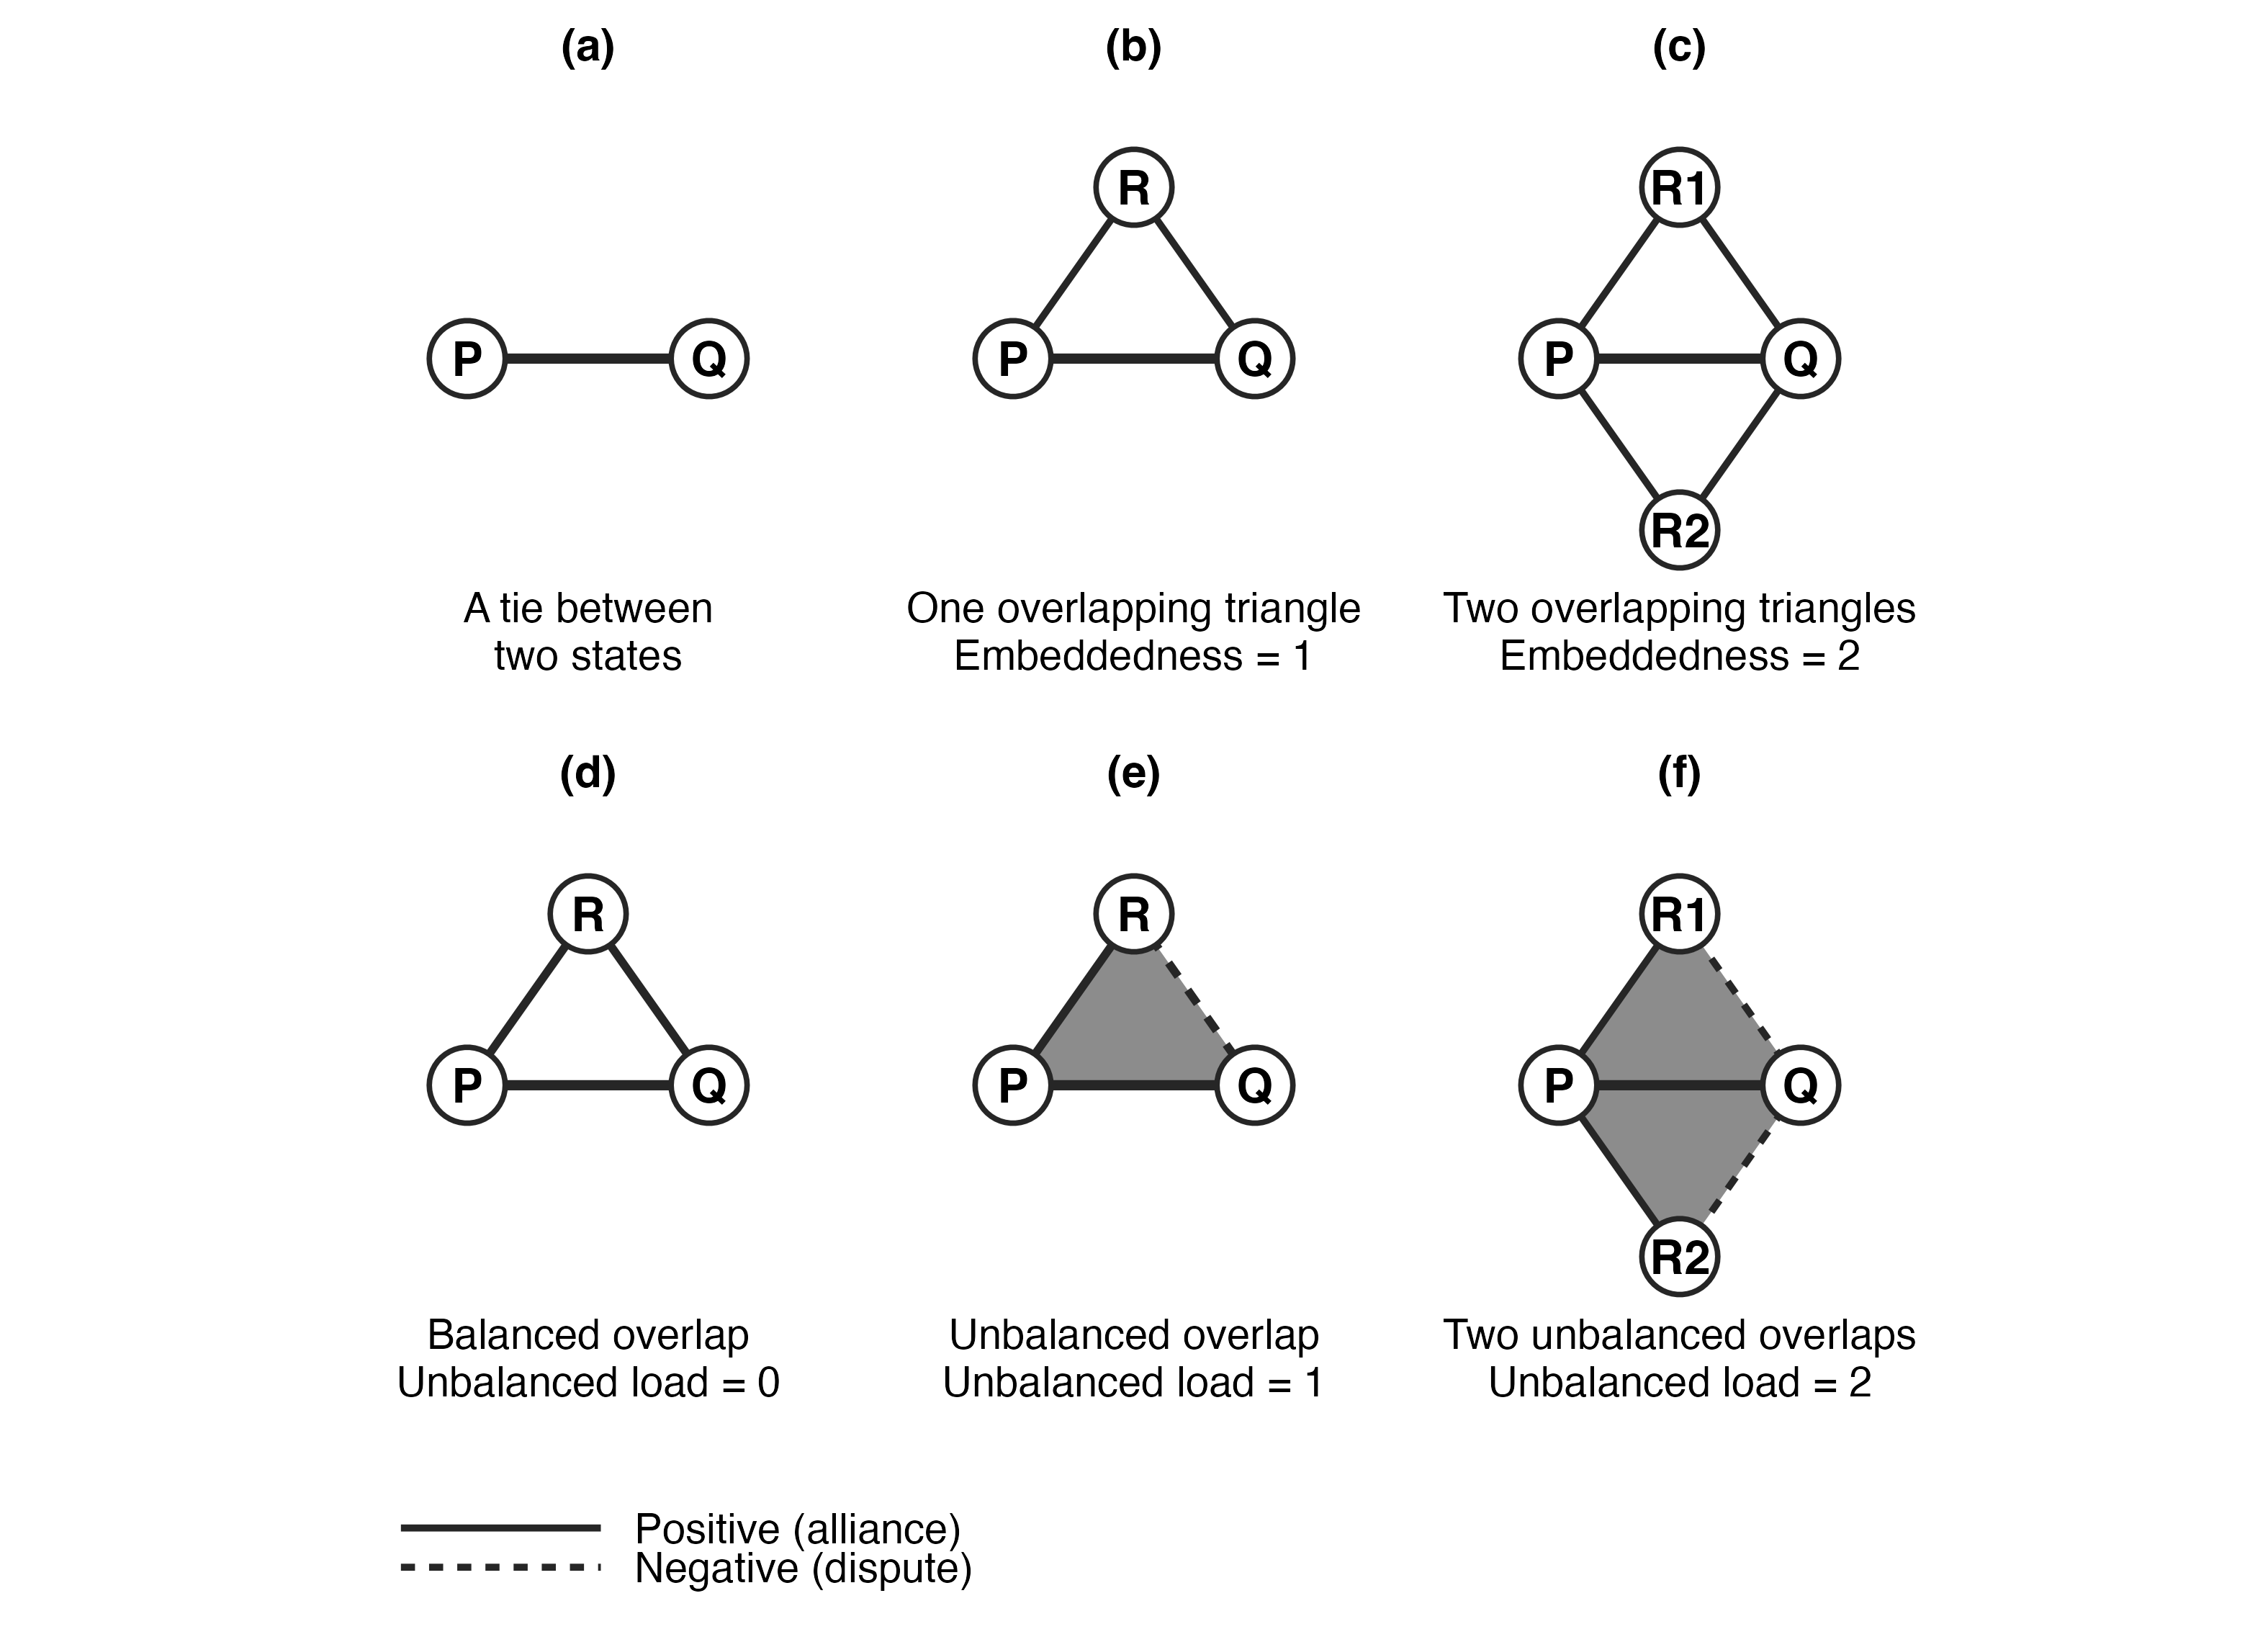
\includegraphics[width=\linewidth]{../../results/fig_schematic_measures.png}

\vspace{4pt}
\textbf{Figure 1. Triadic embeddedness and unbalanced load, illustrated schematically.} (a)--(c) build up embeddedness by adding overlapping triangles around the P--Q tie, regardless of sign. (d)--(f) hold topology fixed and vary triangle sign to isolate unbalanced load: (d)-(e) differ only in the sign of Q--R (balanced, load=0, vs.\ unbalanced, load=1); (f) matches (c)'s two-triangle topology (embeddedness=2) but with both satellite ties negative, so unbalanced load=2. Solid lines are positive (alliance) ties; dashed lines are negative (dispute) ties. See text for full detail.
\end{figure}

\textbf{Robustness controls.} Three further triad-level measures serve as robustness checks, each available only for a subset of the full period. \emph{Trade dependence} (Correlates of War Trade dataset, v4.0; Barbieri, Keshk, and Pollins 2009; Barbieri and Keshk 2016; 1870--2012) is, for each tie, the geometric mean of each state's bilateral trade with its partner as a share of total trade, a proxy for how costly a relationship would be to sever economically, independent of topological embeddedness. \emph{Geographic contiguity} (COW Direct Contiguity, v3.2; Stinnett et al.~2002) is the share of a triad's three dyads sharing a land border or narrow water separation. \emph{Regime type} is the minimum Polity2 score (-10 to +10) across a triad's three members (Polity5; Marshall, Gurr, and Jaggers 2019), the standard ``weakest-link'' operationalization in the joint-democracy literature.

\subsection*{3.3 Competing-risks estimation}

Competing-risks duration models are not new to international relations: Leeds and Savun (2007) use one to distinguish the different ways formal alliances end, and Quiroz Flores (2012) applies the same logic to war termination and leader survival. The contribution here is not the method but the recognition that triadic imbalance has exactly this structure --- an unbalanced triad is continuously exposed to two competing terminal events for as long as it survives, and the question of how long it persists cannot be separated from the question of which event eventually ends it.

\textbf{Setup.} A spell is a unit's continuous exposure to two competing, mutually exclusive terminal events, dissolution and realignment, with right-censoring at 2012 for spells still ongoing --- a classic competing-risks design (Allison 2014), where time spent unbalanced without either event is not an outcome but time still at risk. Each spell is expanded into triad-year form, one row per calendar year at risk, carrying that year's covariates (triadic embeddedness, actor constraint, capability, and, in robustness specifications, trade dependence, contiguity, and regime type), so a spell's risk profile evolves rather than being fixed at onset. This yields 10,170 usable triad-years across 6,176 spells with at least one qualifying at-risk year: 6,097 end in an observed transition (678 dissolution, 5,419 realignment), and 79 are still-censored, contributing only non-terminal at-risk years.

\textbf{Model.} I take a cause-specific hazard approach: for each triad-year $i$ at risk in year $t$, I model the two competing hazards separately as

\begin{multline*}
\Pr(\text{dissolve}_{i,t+1} = 1 \mid \text{at risk}_{i,t}) = \\
\text{logit}^{-1}\big(\beta_0 + \beta_1 E_{i,t} + \beta_2 C_{i,t} + \beta_3 K_{i,t} + \gamma_{\text{era}(t)}\big)
\end{multline*}

and, on the same risk set, the analogous equation for $\Pr(\text{realign}_{i,t+1}=1 \mid \text{at risk}_{i,t})$, where $E_{i,t}$ is triadic embeddedness, $C_{i,t}$ actor constraint, and $K_{i,t}$ capability (log CINC). This is the discrete-time analogue of the Cox cause-specific hazard model: each cause's hazard is estimated on the full risk set, treating triad-years in which the \emph{other} event occurs as not experiencing \emph{this} event that year (coded 0) --- the standard, most directly interpretable approach for the covariate-specific rate of each transition, rather than the cumulative probability of that transition in the presence of the competing risk (what a subdistribution-hazard, or Fine-Gray, specification targets). A logistic link is used rather than complementary log-log, since with annual intervals and hazard probabilities well below where the links diverge, this keeps coefficients on the same footing (log-odds) as the fixed-window robustness models. Standard errors are clustered by triad throughout, since a triad can contribute multiple triad-years and sometimes multiple spells, neither independent.

\textbf{Why not a fixed window.} A natural alternative --- asking whether a triad resolved within, say, 5 years of becoming unbalanced --- was estimated first (online appendix) and points the same direction throughout, but the competing-risks design is primary for two reasons: it avoids justifying an arbitrary window length, since every year of a spell is modeled on its own terms rather than collapsed into a single yes/no outcome; and it uses substantially more data, since a fifteen-year spell contributes fifteen informative triad-year observations rather than one onset-year observation of whether it resolved within an arbitrary window. The two cause-specific logits are estimated separately rather than jointly; a multinomial discrete-time model (persist/dissolve/realign) in the online appendix confirms embeddedness retains the same opposing signs and significance when modeled jointly (Section A12).

\subsection*{3.4 Identification: what these estimates can and cannot claim}

Triadic embeddedness, actor constraint, and unbalanced load are all computed from the same yearly signed network that generates the outcomes being modeled, so the hazard models throughout should be read as \emph{structural associations conditional on a rich set of controls}, not as causal estimates, a standard limitation for observational network analysis. Two checks bound how much it matters: re-estimating with covariates lagged a full year leaves embeddedness's effect essentially unchanged, bounding short-run simultaneity, and a Cinelli and Hazlett (2020) omitted-variable analysis shows an unobserved confounder would need to explain well over 10\% of the residual variance in both embeddedness and the outcome --- more than the paper's own strongest observed control achieves --- to explain the effect away. Neither check addresses the deeper, long-run endogeneity of network structure to decades of prior alliance and dispute politics, which no observational design applied to a single historical system can; what they establish is narrower: the associations are not an artifact of this design's timing choices, nor readily explained by an ordinary confounder. Full detail is in the online appendix (Section A4).

\section*{4. Results}

\subsection*{4.1 Embeddedness reallocates resolution toward realignment}

The trajectories are evident before any model is introduced. Figure 2 follows spells from their onset, grouped by embeddedness at the moment they became unbalanced, and shows what becomes of them over the following twenty years. Among spells beginning in the lowest tercile, the majority end in dissolution within the first few years; among those in the highest tercile, dissolution is rare and the great majority realign quickly, with almost no residual ``still unbalanced'' band by year 10. Spells at intermediate embeddedness show the largest and most persistent residual share of ongoing imbalance, exactly as Section 2 predicts: embeddedness must be high enough to foreclose the low-cost exit through dissolution before it can reliably deliver the higher-effort resolution through realignment, so it is the configurations caught between the two thresholds that persist longest.

\begin{figure*}[t]
\centering
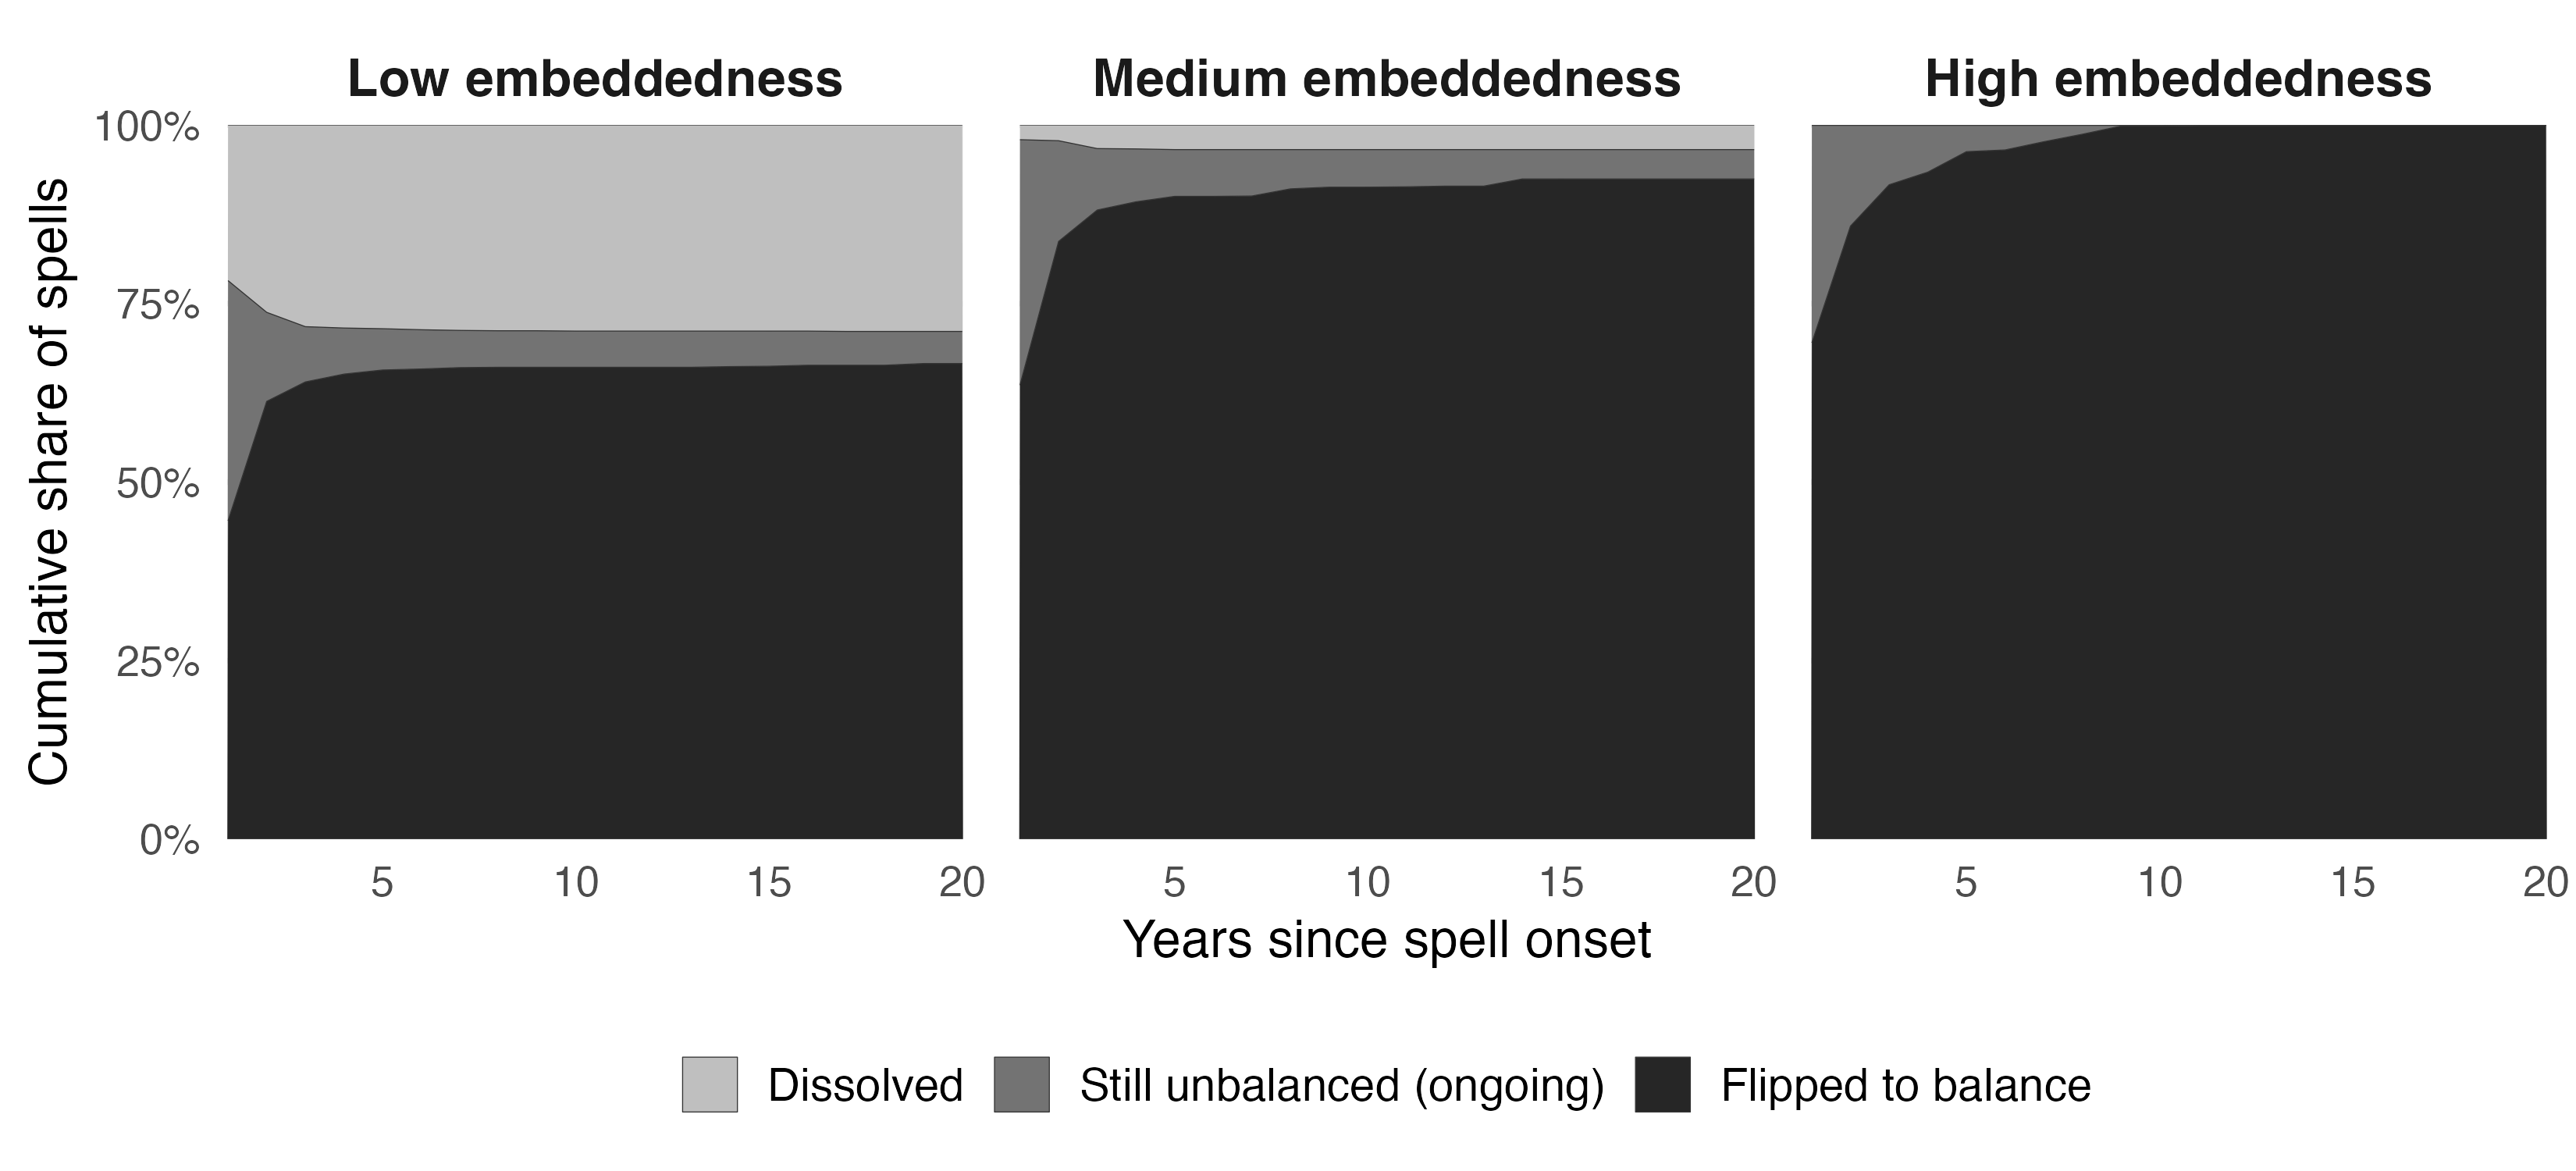
\includegraphics[width=0.92\linewidth]{../../results/fig_cif.png}

\vspace{4pt}
\textbf{Figure 2.} How unbalanced spells end over time (cumulative incidence): dissolved, still ongoing, or realigned, by embeddedness tercile at onset.
\end{figure*}

The competing-risks hazard models test whether this descriptive separation survives controlling for capability, era, and the spell's own duration (fixed effects for years since onset, since Figure 2 suggests transitions cluster early). It does: triadic embeddedness reduces the hazard of dissolution (b=-2.51, SE=0.16, p$<$.001; OR $\approx$ 0.081 per SD, roughly a 92\% reduction) and increases the hazard of realignment (b=+0.44, SE=0.05, p$<$.001; OR $\approx$ 1.55 per SD, roughly a 55\% increase), reported in full in Table 2 (Figure 3); Section 4.5 shows the same direction holds outside major alliance blocs, at different magnitude. Both effects change little without duration fixed effects (online appendix, Section A1); edge betweenness is a much weaker predictor in both hazards (dissolution: b=0.03, p=.63; realignment: b=-0.03, p=.37) --- embeddedness specifically, not bridging position, does the work.

Section 2.2 distinguishes total embeddedness, a triad-level \emph{exposure} measure, from unbalanced load's instantaneous \emph{pressure} (Section 2.3); the interstate network does not contain enough between-triad variation to separate them empirically: triadic embeddedness and current unbalanced load are almost perfectly correlated at the triad-year level (r=0.97), because the unbalanced share of a tie's overlapping triangles is remarkably stable across the embeddedness distribution within this heavily bloc-concentrated risk set. Entering both into the realignment hazard accordingly produces unstable coefficients (VIF $\approx$15, online appendix Section A13), unable to identify whether embeddedness's association with realignment operates through contemporaneous pressure or a distinct exposure mechanism. The cleaner separation occurs within realigning triads, where total embeddedness varies little across the three constituent ties (Section 4.3: 74.6\% of events tied) but unbalanced load varies substantially and predicts which tie changes.

\begin{figure*}[t]
\centering
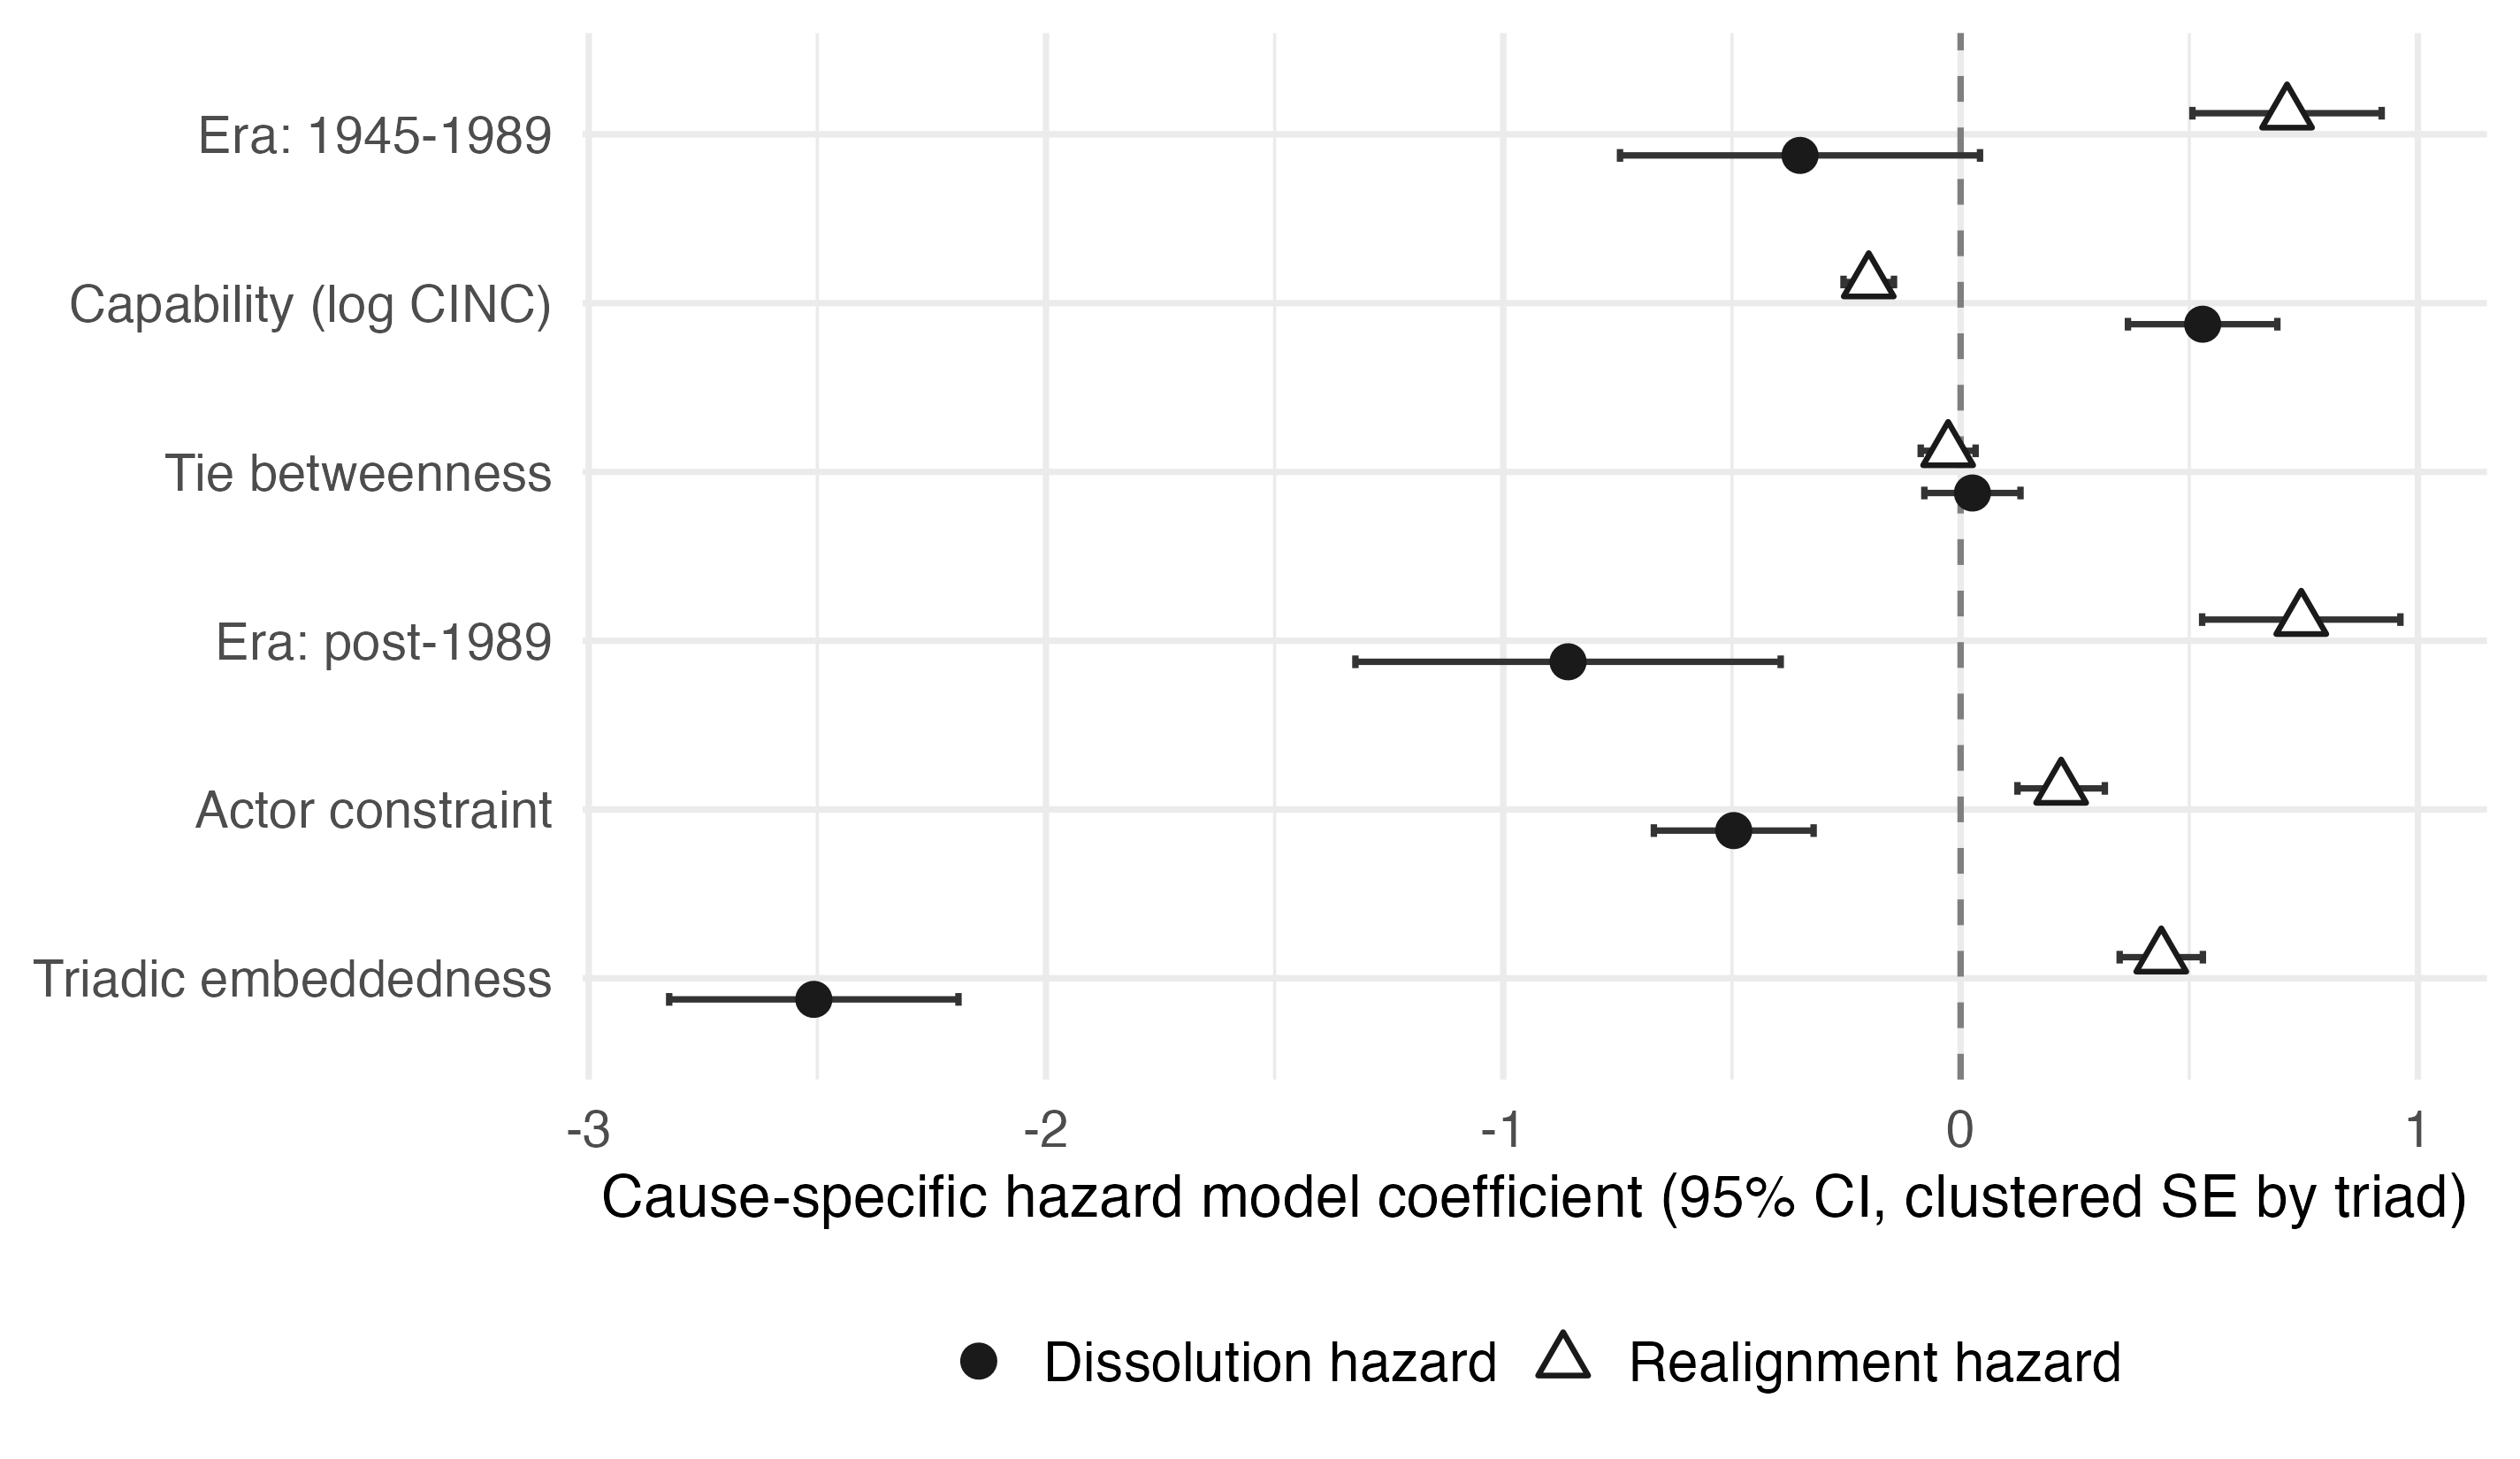
\includegraphics[width=0.75\linewidth]{../../results/fig3_hazard_coefficients.png}

\vspace{4pt}
\textbf{Figure 3.} Cause-specific hazard model coefficients: dissolution vs.~realignment.
\end{figure*}

\begin{table*}[t]
\centering
\textbf{Table 2.} Discrete-time cause-specific hazard models of dissolution and realignment (logistic, clustered SEs by triad). All predictors standardized; OR = odds ratio, the substantive-scale effect of a one-SD increase. A specification without duration fixed effects, and the naive embeddedness-omitted model (Section 4.2), are in the online appendix (Sections A1 and A6).

\vspace{4pt}
{\small\sf
\begin{tabular}{lrrrr}
\toprule
Predictor & Dissolution $b$ (SE) & Dissolution OR & Realignment $b$ (SE) & Realignment OR\\
\midrule
Triadic embeddedness & -2.508*** (0.161) & 0.08 & 0.439*** (0.046) & 1.55\\
Tie betweenness & 0.026 (0.054) & 1.03 & -0.027 (0.031) & 0.97\\
Actor constraint & -0.496*** (0.089) & 0.61 & 0.220*** (0.049) & 1.25\\
Capability (log CINC) & 0.529*** (0.083) & 1.70 & -0.201*** (0.028) & 0.82\\
Era: 1945--1989 & -0.351 (0.201) & 0.70 & 0.714*** (0.106) & 2.04\\
Era: post-1989 & -0.858*** (0.237) & 0.42 & 0.745*** (0.111) & 2.11\\
Duration: year 2 & -0.403** (0.148) & 0.67 & -0.118* (0.053) & 0.89\\
Duration: year 3 & 0.827*** (0.203) & 2.29 & -0.938*** (0.084) & 0.39\\
Duration: years 4--5 & -1.788*** (0.406) & 0.17 & -1.492*** (0.086) & 0.22\\
Duration: years 6--10 & -1.750*** (0.411) & 0.17 & -1.872*** (0.100) & 0.15\\
Duration: years 11+ & -2.598** (0.959) & 0.07 & -1.737*** (0.114) & 0.18\\
Intercept & -4.020*** (0.261) & --- & -0.246* (0.104) & ---\\
N (triad-years) & 10,170 & & 10,170 & \\
\bottomrule
\end{tabular}
\par}

\vspace{4pt}
{\small *p$<$.05, **p$<$.01, ***p$<$.001. Reference category for era: pre-1945; reference category for duration: spell's first year at risk.}
\end{table*}

\subsection*{4.2 A supplementary structural result: actor constraint}

Actor-level constraint (Burt 1992), estimated jointly with triadic embeddedness (Table 2), reduces the dissolution hazard and increases the realignment hazard in the same direction as embeddedness (b=-0.50 and b=+0.22, both p$<$.001) --- evidence that position-level and relation-level structural constraint operate as parallel, reinforcing mechanisms once properly separated. Omitting embeddedness recovers the \emph{opposite sign} on both hazards, since the two are substantially negatively correlated (r=-0.78): high-degree states brokering the most overlapping relationships mechanically register \emph{low} Burt constraint. This is a specification lesson, not a third contribution alongside H1 and H2; the naive comparison is in the online appendix (Section A6).

\subsection*{4.3 Within a realigning triad, the tie under the most unbalanced-triad pressure is the one that changes}

H1 concerns which triads realign; H2 asks which specific tie changes when one does. Testing this requires identifying, for every realignment event, which of the triad's three ties actually changed sign --- 5,414 of 5,419 realignment events (99.9\%) involve exactly one, giving a clean three-way choice per event.

Unbalanced load, not total embeddedness, is the measure that does this work. Total embeddedness counts every triangle a tie is embedded in regardless of whether those triangles are unbalanced, and 74.6\% of realignment events have exactly tied total embeddedness across all three of a triad's edges --- a direct consequence of the alliance-bloc concentration in Section 4.5 --- leaving too little variation and no significant pattern in what remains. Unbalanced load varies far more: only 0.1\% of events have it exactly tied, leaving 2,516 events (46.5\%) with all three values distinct, and among these, the tie that changes has the \emph{highest} unbalanced load in 96.6\% of events, against a 33.3\% chance baseline (p$<$.001). A conditional logit confirms this with a large, precisely estimated coefficient (odds ratio $\approx$ 1.38 per unit, p$<$.001), essentially unchanged when total embeddedness and betweenness are added as controls.

This pooled figure needs one qualification: in the dominant two-positive-one-negative configuration, the negative tie is definitionally the edge shared by every unbalanced triangle, so it is structurally the likeliest candidate regardless of mechanism --- a bare negative-tie indicator alone predicts nearly as well (concordance 0.977 vs.\ 0.975). The cleaner, same-sign-pairs test, where a sign indicator carries no information, still finds the higher-unbalanced-load tie changes in 75.2\% of cases (n=137, p$<$.001 against a 50\% null, robust to dyad-year dependence). Unbalanced load therefore predicts tie choice beyond current sign; full detail is in the online appendix (Section A12).

The results form a coherent account across three levels: triadic embeddedness predicts \emph{whether} a triad realigns (H1); a tie's unbalanced load predicts, beyond tie sign alone, \emph{which} tie realigns when it does (H2); and actor-level constraint (Section 4.2) operates in the same direction as embeddedness once properly separated from it.

\begin{table*}[t]
\centering
\textbf{Table 3.} Conditional logit, within-triad tie choice at realignment (3 ties as alternatives, stratified by event). Fit on all 5,414 single-tie-change events (the text's binomial test uses the 2,516-event subsample with all three ties' unbalanced load distinct; the conditional logit's exact partial-likelihood method handles ties directly).

\vspace{4pt}
{\small\sf
\begin{tabular}{lrr}
\toprule
Predictor & Unbalanced load only & With controls\\
\midrule
Unbalanced load & 0.320*** (0.008) & 0.322*** (0.009)\\
Triadic embeddedness & --- & -0.064* (0.027)\\
Tie betweenness & --- & 0.001 (0.001)\\
N (tie-alternatives) & 16,242 & 16,242\\
N (events) & 5,414 & 5,414\\
Concordance & 0.975 & 0.977\\
\bottomrule
\end{tabular}
\par}

\vspace{4pt}
{\small *p$<$.05, ***p$<$.001. Concordance is the standard coxph-family statistic (the conditional logit is fit as a stratified Cox model): the share of comparable tie-pairs within an event for which the model ranks the higher-unbalanced-load tie more likely to change.}
\end{table*}

Does this pattern hold equally for alliance-to-hostility and hostility-to-alliance realignment? These are not symmetric events substantively --- one is a formal commitment's failure, the other its formation. Of the 2,516 events with all three ties' unbalanced load distinct, 67 (2.7\%) are alliance-to-hostility and 2,449 (97.3\%) are hostility-to-alliance, so the pooled 96.6\% figure above is overwhelmingly a statement about the latter. Splitting the test by tie type (Table 4) shows the two diverge sharply: among hostility-to-alliance events, unbalanced load performs even better than the pooled estimate (highest load in 98.9\% of cases, n=2,449), while among alliance-to-hostility events the pattern reverses, with the changed tie carrying the highest load in only 11.9\% of cases (n=67), significantly \emph{below} the 33.3\% chance baseline ($\chi^2$=1467.5, df=1, p$<$.001).

\begin{table*}[t]
\centering
\textbf{Table 4.} Unbalanced-load hit rate (changed tie has the maximum value among the triad's three ties), by changed-tie type. Restricted to the 2,516 events with all three ties' unbalanced load distinct; null hit rate under chance is 33.3\%.

\vspace{4pt}
{\small\sf
\begin{tabular}{lrrrr}
\toprule
Group & N & Hit rate & 95\% CI & p (vs.~1/3 baseline)\\
\midrule
All events & 2,516 & 96.6\% & [95.8\%, 97.3\%] & $<$.001\\
Alliance-to-hostility (pos $\rightarrow$ neg) & 67 & 11.9\% & [5.3\%, 22.2\%] & $<$.001\\
Hostility-to-alliance (neg $\rightarrow$ pos) & 2,449 & 98.9\% & [98.4\%, 99.3\%] & $<$.001\\
\bottomrule
\end{tabular}
\par}
\end{table*}

The reversal is not an artifact of alliance-to-hostility events starting from a different triad configuration: essentially all of them (67 of 67) begin, like hostility-to-alliance events, from the same two-positive-one-negative configuration, with only 5 residual zero-positive-three-negative events, all on the hostility-to-alliance side, too few to explain the reversal (full cross-tab in the online appendix, Section A12). Whatever distinguishes the two tie types, it is not which triad shape they start from.

A conditional logit with an unbalanced-load $\times$ tie-type interaction, fit on the full 5,414-event sample (16,242 tie-alternatives, matching Table 3), estimates the interaction as small and not statistically distinguishable from zero (b=-0.023, SE=0.044, p=.60; LRT $\chi^2$=0.28, df=1, p=.60), even though the tie-type main effect is large and significant (b=-2.44, SE=0.14, p$<$.001). This is best read as a striking descriptive boundary condition (Table 4) the data cannot formally establish as moderation: unbalanced load predicts tie choice almost deterministically for the dominant transition type, hostility-to-alliance, while the much smaller alliance-to-hostility subsample reverses. Both are substantive relational reclassifications, so the asymmetry needs a different account; one possibility is that transitions into hostility face additional bilateral and domestic constraints that transitions toward alignment do not (Leeds and Savun 2007; Fearon 1994). The pooled 96.6\% figure is accordingly a strong finding about hostility-to-alliance realignment specifically, not a general law confirmed across both directions.

\subsection*{4.4 The modal dissolution event is a dispute lapsing, not an alliance expiring or a state disappearing}

Treating ``dissolution'' as a single category risks pooling substantively different processes --- an alliance's term ending, a militarized dispute simply not recurring, or a state exiting the interstate system entirely. Disaggregating the 678 dissolution events shows the modal case is specifically a militarized dispute not being renewed: among the 407 single-tie disappearances (60.0\% of all dissolution events), 80.1\% are a lapsed dispute and only 19.9\% an unrenewed alliance, with none coinciding with a state exiting the system (full breakdown in the online appendix, Section A10). This is closer to what the rivalry- and alliance-termination literatures already study under different names (Leeds and Savun 2007) than to alliance expiration or state death, though not equivalent to rivalry termination in that literature's own sense: a rivalry can encompass many separate MIDs, and the negative-tie coding here is deliberately dispute-level, as the triad-year design requires. Section 5 treats the connection accordingly, as a neighboring implication rather than a direct measurement (Bennett 1997).

\subsection*{4.5 Robustness}

Three further checks (online appendix, Sections A2, A3, A11) confirm the primary results are robust. Trade dependence (1870--2012 subsample) is itself a significant predictor in both hazards, but does not absorb embeddedness's effect, which retains its full strength (b=-2.46 dissolution, b=+0.37 realignment). Adding geographic contiguity and regime type (restricted Polity5 subsample) leaves embeddedness and actor constraint intact, with a fixed 5-year-window benchmark reproducing the same pattern. And the alliance system's concentration into major 20th- and 21st-century blocs (87.6\% of triad-years) --- also a dependence problem, addressed directly in Section 5 --- does not undermine the embeddedness effect, which survives excluding bloc-touching spells, controlling for bloc membership, or two-way clustering standard errors by triad and bloc.

\section*{5. Discussion}

Embeddedness supplies the explanation this paper set out to test: weakly embedded inconsistencies mostly disappear, strongly embedded ones mostly get realigned, and it is only the intermediate range where genuine persistence concentrates. Particular dynamic formulations of balance theory treat a tie as a fixed feature that can only be flipped (Antal, Krapivsky, and Redner 2005; Marvel et al.~2011), a modeling choice, not an inherent commitment of balance theory as such (Section 2.1); allowing for dissolution is what distinguishes which trajectory a given episode of imbalance takes. A substantial share of this evidence comes from ties inside major multilateral alliance blocs (NATO, the Warsaw Pact, the Rio Pact), but the direction holds outside them too (Section 4.5), decomposing unevenly: outside blocs, embeddedness's effect on dissolution is smaller (b=-0.78) but larger on realignment (b=+1.10) than the full-sample estimate, while inside blocs the pattern reverses (effective b=-2.03 dissolution, b=+0.33 realignment; online appendix, Section A2) --- formal institutionalization mainly amplifies durability once embedded, not whether embeddedness drives realignment.

Three implications follow. First, for balance theory itself: balance is not simply produced by sign-switching. Particular dynamic formulations model every unbalanced triad as eventually resolving through a flipped tie, but a large share of the triads here resolve instead by a tie disappearing, and which happens is systematically predicted by structure --- down to which specific tie moves within a realigning triad (Section 4.3), extending Rawlings and Friedkin's (2017) balance-violation exposure mechanism to a within-event choice among a triad's three relationships. The actor-constraint result (Section 4.2) adds a related point: correlated measures need to be estimated jointly, since dropping either recovers a misleadingly reversed coefficient on the other. Second, for what ``persistence'' means: a configuration that looks anomalously durable in a model tracking only realignment is not necessarily evidence balance pressure has failed. It can instead occupy the region between a viable exit and a viable adaptation --- embedded enough that dissolution is no longer low-cost, but not so embedded that realignment is yet reliably available.

Third, for international relations specifically, this connects the triadic, network-structural logic of balance theory to two literatures already introduced in Section 2.1, extra-dyadic IR network research and the dyadic rivalry- and alliance-termination literatures, that have each captured part of the picture without the other half. This paper's contribution sits at the intersection: embeddedness predicts which of the two dyadic exits a given episode of inconsistency takes, and which specific tie carries the realignment when that is the exit taken --- related but distinct claims, since H1 concerns variation between triads while H2 concerns variation among ties within triads that realign. Dense triadic embeddedness is plausibly a structural precondition for the kind of dramatic bilateral realignment that can end a rivalry outright (the introduction's Britain-USSR case), and for alliance termination, abrogation likely grows structurally costly inside a dense multilateral bloc since exit disturbs every relationship built on the same foundation --- both offered as connections rather than claims tested here (Section 4.4; Bennett 1997; Leeds and Savun 2007). A tie's embeddedness should predict not just \emph{whether} it ends, but \emph{how}, a bridge for future work that likely needs to treat ``realignment'' as two distinct processes rather than one, given how sharply alliance-to-hostility and hostility-to-alliance realignment diverge (Section 4.3).

Several limitations bound these conclusions. Unbalanced load is measured on the same observed network used to define the triads and spells themselves, rather than through a design holding network structure exogenous to the dynamics explained. At the edge level used in H2, it is also, by construction, correlated with total embeddedness (r=0.33) and with actor-level constraint --- a different quantity from the r=0.97 triad-year-level correlation in Section 4.1, since the two are computed on different units (edges within events versus triad-year means across the risk set). The conditional logit shows its effect survives controlling for both, but an independent test on a different signed network would strengthen confidence the mechanism is specifically about unresolved pressure rather than general local density.

H1's dependence structure raises a concern analogous to H2's in Section 4.3: a single tie change can end many overlapping spells at once, and triad-clustered standard errors alone do not capture dependence from shared dyads, states, or bloc membership. Section 4.5's two-way-clustered specification bounds this: embeddedness's effect remains correctly signed and significant once bloc-level dependence is modeled explicitly, though standard errors roughly double --- bounding rather than eliminating the concern that the panel's 6,277 nominal spells overstate the independent information behind the reported estimates.

The triad population is necessarily built from realized alliance and dispute ties, so small or peripheral states with no signed relationships in a given period are invisible to the analysis. Every measure here is also built on a one-mode projection that treats a multilateral alliance like a bilateral treaty; Appendix A2 shows the results are robust to, but not entirely independent of, the resulting concentration in major blocs. A two-mode representation, with organizations as a second node type, would be more faithful to Heider's (1946) original formulation, and a proxy for it (Appendix A3) points the same direction; Fritz et al.'s (2025) dynamic signed exponential-random-graph model offers one plausible framework for the full redesign.

The H2 heterogeneity between alliance-to-hostility and hostility-to-alliance realignment rests on a small alliance-to-hostility subsample (n=67); the descriptive gap is large, but the formal interaction test cannot confirm it as moderation on its own, and a larger sample --- plausibly requiring data beyond the interstate system --- would be needed to establish it as a general property rather than a suggestive pattern here.

Both the embeddedness and actor-constraint results, while robust across every specification tested here (fixed-window and competing-risks alike, with and without duration, trade, contiguity, and regime-type controls), were developed on the same historical dataset; independent replication on signed networks outside the interstate system would strengthen confidence that ``exit versus realignment'' is a general property of relational systems under structural constraint, not one specific to interstate data.

None of this changes the paper's central empirical claim. Unbalanced triads in the interstate system exit through dissolution or realignment, the route taken varies systematically with triadic embeddedness, and getting this right requires recognizing exit as a theoretically meaningful outcome rather than folding it into an undifferentiated ``did not resolve'' category. Some hostile ties end because nothing held them in place; overwhelmingly, the evidence here suggests, a militarized dispute was simply not renewed, not a state disappearing or an alliance's term expiring. Others end in realignment because too much held them in place for exit to be an option. The apparent persistence in between is not a third kind of ending. It is simply time still at risk of one of the other two, so persistence can emerge without any mechanism that positively sustains imbalance. It arises because the two processes that terminate imbalance dominate in different parts of the structural landscape, a claim about how competing exits interact that does not depend on the interstate system specifically and should travel to other relational systems under structural constraint.

\section*{Data Availability Statement}

Replication code and data are available at \url{https://anonymous.4open.science/r/two-paths-out-of-imbalance/} (anonymized for double-blind review).

\begin{thebibliography}{99}

\bibitem[Allison(2014)]{Allison2014} Allison, Paul D. 2014. \emph{Event History and Survival Analysis}, 2nd ed. Sage.

\bibitem[Antal, Krapivsky, and Redner(2005)]{Antal2005} Antal, T., P. L. Krapivsky, and S. Redner. 2005. ``Dynamics of Social Balance on Networks.'' \emph{Physical Review E} 72(3): 036121.

\bibitem[Barbieri and Keshk(2016)]{Barbieri2016} Barbieri, Katherine, and Omar Keshk. 2016. \emph{Correlates of War Project Trade Data Set Codebook, Version 4.0.}

\bibitem[Barbieri, Keshk, and Pollins(2009)]{Barbieri2009} Barbieri, Katherine, Omar M. G. Keshk, and Brian Pollins. 2009. ``Trading Data: Evaluating Our Assumptions and Coding Rules.'' \emph{Conflict Management and Peace Science} 26(5): 471--491.

\bibitem[Bennett(1996)]{Bennett1996} Bennett, D. Scott. 1996. ``Security, Bargaining, and the End of Interstate Rivalry.'' \emph{International Studies Quarterly} 40(2): 157--183.

\bibitem[Bennett(1997)]{Bennett1997} Bennett, D. Scott. 1997. ``Measuring Rivalry Termination, 1816--1992.'' \emph{Journal of Conflict Resolution} 41(2): 227--254.

\bibitem[Burt(1992)]{Burt1992} Burt, Ronald S. 1992. \emph{Structural Holes: The Social Structure of Competition.} Harvard University Press.

\bibitem[Caimo and Gollini(2026)]{Caimo2026} Caimo, Alberto, and Isabella Gollini. 2026. ``Separable Models for Dynamic Signed Networks.'' \emph{Journal of the Royal Statistical Society, Series A}, advance access. DOI: 10.1093/jrsssa/qnag053.

\bibitem[Cartwright and Harary(1956)]{Cartwright1956} Cartwright, Dorwin, and Frank Harary. 1956. ``Structural Balance: A Generalization of Heider's Theory.'' \emph{Psychological Review} 63(5): 277--293.

\bibitem[Cinelli and Hazlett(2020)]{Cinelli2020} Cinelli, Carlos, and Chad Hazlett. 2020. ``Making Sense of Sensitivity: Extending Omitted Variable Bias.'' \emph{Journal of the Royal Statistical Society, Series B (Statistical Methodology)} 82(1): 39--67.

\bibitem[Colaresi, Rasler, and Thompson(2007)]{Colaresi2007} Colaresi, Michael P., Karen Rasler, and William R. Thompson. 2007. \emph{Strategic Rivalries in World Politics: Position, Space and Conflict Escalation.} Cambridge University Press.

\bibitem[Coleman(1988)]{Coleman1988} Coleman, James S. 1988. ``Social Capital in the Creation of Human Capital.'' \emph{American Journal of Sociology} 94: S95--S120.

\bibitem[Corbetta and Grant(2012)]{Corbetta2012} Corbetta, Renato, and Keith A. Grant. 2012. ``Intervention in Conflicts from a Network Perspective.'' \emph{Conflict Management and Peace Science} 29(3): 314--340.

\bibitem[Cranmer, Desmarais, and Kirkland(2012)]{CranmerKirkland2012} Cranmer, Skyler J., Bruce A. Desmarais, and Justin H. Kirkland. 2012. ``Toward a Network Theory of Alliance Formation.'' \emph{International Interactions} 38(3): 295--324.

\bibitem[Cranmer, Desmarais, and Menninga(2012)]{Cranmer2012} Cranmer, Skyler J., Bruce A. Desmarais, and Elizabeth J. Menninga. 2012. ``Complex Dependencies in the Alliance Network.'' \emph{Conflict Management and Peace Science} 29(3): 279--313.

\bibitem[Davis(1967)]{Davis1967} Davis, James A. 1967. ``Clustering and Structural Balance in Graphs.'' \emph{Human Relations} 20(2): 181--187.

\bibitem[Diaz-Diaz, Bartesaghi, and Estrada(2024)]{DiazDiaz2024} Diaz-Diaz, Fernando, Paolo Bartesaghi, and Ernesto Estrada. 2024. ``Mathematical Modeling of Local Balance in Signed Networks and Its Applications to Global International Analysis.'' \emph{Journal of Applied Mathematics and Computing} 70: 6195--6218.

\bibitem[Diehl and Goertz(2000)]{Diehl2000} Diehl, Paul F., and Gary Goertz. 2000. \emph{War and Peace in International Rivalry.} University of Michigan Press.

\bibitem[Dixon(1994)]{Dixon1994} Dixon, William J. 1994. ``Democracy and the Peaceful Settlement of International Conflict.'' \emph{American Political Science Review} 88(1): 14--32.

\bibitem[Doreian and Krackhardt(2001)]{Doreian2001} Doreian, Patrick, and David Krackhardt. 2001. ``Pre-Transitive Balance Mechanisms for Signed Networks.'' \emph{Journal of Mathematical Sociology} 25(1): 43--67.

\bibitem[Doreian and Mrvar(2015)]{DoreianMrvar2015} Doreian, Patrick, and Andrej Mrvar. 2015. ``Structural Balance and Signed International Relations.'' \emph{Journal of Social Structure} 16: 1--49.

\bibitem[Fearon(1994)]{Fearon1994} Fearon, James D. 1994. ``Domestic Political Audiences and the Escalation of International Disputes.'' \emph{American Political Science Review} 88(3): 577--592.

\bibitem[Fritz et al.(2025)]{Fritz2025} Fritz, Cornelius, Marius Mehrl, Paul W. Thurner, and G\"oran Kauermann. 2025. ``Exponential Random Graph Models for Dynamic Signed Networks: An Application to International Relations.'' \emph{Political Analysis} 33: 211--230.

\bibitem[Gallo et al.(2024)]{Gallo2024} Gallo, Anna, Diego Garlaschelli, Renaud Lambiotte, Fabio Saracco, and Tiziano Squartini. 2024. ``Testing Structural Balance Theories in Heterogeneous Signed Networks.'' \emph{Communications Physics} 7: 154.

\bibitem[Gibler(2009)]{Gibler2009} Gibler, Douglas M. 2009. \emph{International Military Alliances, 1648--2008.} CQ Press.

\bibitem[Granovetter(1985)]{Granovetter1985} Granovetter, Mark. 1985. ``Economic Action and Social Structure: The Problem of Embeddedness.'' \emph{American Journal of Sociology} 91(3): 481--510.

\bibitem[Heider(1946)]{Heider1946} Heider, Fritz. 1946. ``Attitudes and Cognitive Organization.'' \emph{Journal of Psychology} 21(1): 107--112.

\bibitem[Hummon and Doreian(2003)]{Hummon2003} Hummon, Norman P., and Patrick Doreian. 2003. ``Some Dynamics of Social Balance Processes: Bringing Heider Back Into Balance Theory.'' \emph{Social Networks} 25(1): 17--49.

\bibitem[Kinne(2024)]{Kinne2024} Kinne, Brandon J. 2024. ``Network Context and the Effectiveness of International Agreements.'' \emph{International Studies Quarterly} 68(3): sqae099.

\bibitem[Krackhardt(1998)]{Krackhardt1998} Krackhardt, David. 1998. ``Simmelian Ties: Super Strong and Sticky.'' In \emph{Power and Influence in Organizations}, ed. Roderick M. Kramer and Margaret A. Neale, 21--38. Thousand Oaks, CA: Sage.

\bibitem[Larson(2021)]{Larson2021} Larson, Jennifer M. 2021. ``Networks of Conflict and Cooperation.'' \emph{Annual Review of Political Science} 24: 89--107.

\bibitem[Leeds and Savun(2007)]{Leeds2007} Leeds, Brett Ashley, and Burcu Savun. 2007. ``Terminating Alliances: Why Do States Abrogate Agreements?'' \emph{Journal of Politics} 69(4): 1118--1132.

\bibitem[Lerner(2016)]{Lerner2016} Lerner, J\"urgen. 2016. ``Structural Balance in Signed Networks: Separating the Probability to Interact from the Tendency to Fight.'' \emph{Social Networks} 45: 66--77.

\bibitem[Leskovec, Huttenlocher, and Kleinberg(2010)]{Leskovec2010} Leskovec, Jure, Daniel Huttenlocher, and Jon Kleinberg. 2010. ``Signed Networks in Social Media.'' \emph{Proceedings of the SIGCHI Conference on Human Factors in Computing Systems}, 1361--1370.

\bibitem[Maoz et al.(2007)]{Maoz2007} Maoz, Zeev, Lesley G. Terris, Ranan D. Kuperman, and Ilan Talmud. 2007. ``What Is the Enemy of My Enemy? Causes and Consequences of Imbalanced International Relations, 1816--2001.'' \emph{Journal of Politics} 69(1): 100--115.

\bibitem[Maoz and Russett(1993)]{Maoz1993} Maoz, Zeev, and Bruce Russett. 1993. ``Normative and Structural Causes of Democratic Peace, 1946-1986.'' \emph{American Political Science Review} 87(3): 624--638.

\bibitem[Maoz et al.(2019)]{Maoz2019} Maoz, Zeev, Paul L. Johnson, Jasper Kaplan, Fiona Ogunkoya, and Aaron P. Shreve. 2019. ``The Dyadic Militarized Interstate Disputes (MIDs) Dataset Version 3.0: Logic, Characteristics, and Comparisons to Alternative Datasets.'' \emph{Journal of Conflict Resolution} 63(3): 811--835.

\bibitem[Marshall, Gurr, and Jaggers(2019)]{Marshall2019} Marshall, Monty G., Ted Robert Gurr, and Keith Jaggers. 2019. \emph{Polity5: Political Regime Characteristics and Transitions, 1800-2018.} Center for Systemic Peace.

\bibitem[Marvel et al.(2011)]{Marvel2011} Marvel, Seth A., Jon Kleinberg, Robert D. Kleinberg, and Steven H. Strogatz. 2011. ``Continuous-Time Model of Structural Balance.'' \emph{Proceedings of the National Academy of Sciences} 108(5): 1771--1776.

\bibitem[Oishi and Sakuwa(2025)]{Oishi2025} Oishi, Koji, and Kentaro Sakuwa. 2025. ``Structural Balance of Alliance and Rivalry Networks in International Relations.'' \emph{Artificial Life and Robotics} 30: 303--309.

\bibitem[Polidoro, Ahuja, and Mitchell(2011)]{Polidoro2011} Polidoro, Francisco, Jr., Gautam Ahuja, and Will Mitchell. 2011. ``When the Social Structure Overshadows Competitive Incentives: The Effects of Network Embeddedness on Joint Venture Dissolution.'' \emph{Academy of Management Journal} 54(1): 203--223.

\bibitem[Prins and Daxecker(2008)]{Prins2008} Prins, Brandon C., and Ursula E. Daxecker. 2008. ``Committed to Peace? Liberal Institutions and the Termination of Rivalry.'' \emph{British Journal of Political Science} 38(1): 17--34.

\bibitem[Quiroz Flores(2012)]{Quiroz2012} Quiroz Flores, Alejandro. 2012. ``A Competing Risks Model of War Termination and Leader Change.'' \emph{International Studies Quarterly} 56(4): 809--819.

\bibitem[Rawlings and Friedkin(2017)]{Rawlings2017} Rawlings, Craig M., and Noah E. Friedkin. 2017. ``The Structural Balance Theory of Sentiment Networks: Elaboration and Test.'' \emph{American Journal of Sociology} 123(2): 510--548.

\bibitem[Sakuwa and Thompson(2019)]{Sakuwa2019} Sakuwa, Kentaro, and William R. Thompson. 2019. ``On the Origins, Persistence and Termination of Spatial and Positional Rivalries in World Politics: Elaborating a Two-Issue Theory of Conflict Escalation.'' \emph{International Area Studies Review} 22(3): 203--225.

\bibitem[Sarkees and Wayman(2010)]{Sarkees2010} Sarkees, Meredith Reid, and Frank Wayman. 2010. \emph{Resort to War: A Data Guide to Inter-State, Extra-State, Intra-State, and Non-State Wars, 1816--2007.} CQ Press.

\bibitem[Singer, Bremer, and Stuckey(1972)]{Singer1972a} Singer, J. David, Stuart Bremer, and John Stuckey. 1972. ``Capability Distribution, Uncertainty, and Major Power War, 1820--1965.'' In \emph{Peace, War, and Numbers}, ed. Bruce Russett, 19--48. Sage.

\bibitem[Singer and Small(1972)]{Singer1972b} Singer, J. David, and Melvin Small. 1972. \emph{The Wages of War, 1816--1965: A Statistical Handbook.} New York: John Wiley and Sons.

\bibitem[Stinnett et al.(2002)]{Stinnett2002} Stinnett, Douglas M., Jaroslav Tir, Philip Schafer, Paul F. Diehl, and Charles Gochman. 2002. ``The Correlates of War Project Direct Contiguity Data, Version 3.'' \emph{Conflict Management and Peace Science} 19(2): 58--66.

\bibitem[Thompson(2022)]{Thompson2022} Thompson, William R. 2022. ``Constructing a General Model Accounting for Interstate Rivalry Termination.'' In William R. Thompson, Kentaro Sakuwa, and Prashant Hosur Suhas, \emph{Analyzing Strategic Rivalries in World Politics: Types of Rivalry, Regional Variation, and Escalation/De-escalation}, ch.~13. Palgrave Macmillan.

\bibitem[Uzzi(1997)]{Uzzi1997} Uzzi, Brian. 1997. ``Social Structure and Competition in Interfirm Networks: The Paradox of Embeddedness.'' \emph{Administrative Science Quarterly} 42(1): 35--67.

\bibitem[van de Rijt(2011)]{VandeRijt2011} van de Rijt, Arnout. 2011. ``The Micro-Macro Link for the Theory of Structural Balance.'' \emph{Journal of Mathematical Sociology} 35(1--3): 94--113.

\bibitem[Warren(2010)]{Warren2010} Warren, T. Camber. 2010. ``The Geometry of Security: Modeling Interstate Alliances as Evolving Networks.'' \emph{Journal of Peace Research} 47(6): 697--709.

\end{thebibliography}

\end{document}
